\documentclass{book}
\usepackage[subpreambles=false]{standalone}

%%%%%%%%%%%%%%%%%%%%%%%%%%%
% Silence warning messages
\usepackage{silence}
\WarningsOff[scrlayer-notecolumn]
\WarningsOff[biblatex]

%%%%%%%%%%%%%%%%%%%%
% Commenting

%\usepackage[author=Lyndon]{pdfcomment}
%\newcommand{\pdfcomment}[1]{} %ignore all comments

%\usepackage{todonotes}
%\newcommand{\pdfcomment}{\todo}


%%%%%%%%%%%%%%%%%%%%
% Tables
\usepackage{booktabs}

%%%%%%%%%%%%%%%%%%%
% Fonts
\usepackage{tgadventor} %sans
\usepackage{tgpagella}  %serif
\usepackage{inconsolata} %mono
\usepackage[T1]{fontenc}

\usepackage{microtype}
\usepackage[all]{nowidow}
%%%%%%%%%%%%%%%%%%%%%%%
% Styling
\setcounter{secnumdepth}{4}
\setcounter{tocdepth}{2}

\usepackage{placeins}



%%%%%%%%%%%%%%%%%%%
% Math
\usepackage{amsmath, amssymb, stmaryrd, mathtools}
\DeclareMathOperator*{\argmin}{argmin}
\DeclareMathOperator*{\argmax}{argmax}

\usepackage{xparse,xstring,etoolbox}
% crossref this against notation section
\newcommand{\vv}[1]{\tilde{#1}} % vector
\newcommand{\seq}[1]{\mathcal{#1}} % sequence
\newcommand{\set}[1]{\mathbb{#1}} % set

%%%%%%%%%
% Indexing/sequence indexing
\newcommand{\seqind}[2]{#1^{#2}} % seqence index
\newcommand{\ind}[2]{#1_{#2}} % indexed
\newcommand{\disamb}[2]{#1^{\mathrm{#2}}} %disambiguated

%% Smart indexing and naming
\newcommand{\ifupper}[3]{
    \normalexpandarg
	\exploregroups
	\StrCount{ABCDEFGHIJKLMNOPQRSTUVWXYZ}{#1}[\uppercount]
	\ifnumgreater{\uppercount}{0}{#2}{#3}
}

%smart index
\DeclareDocumentCommand{\ii}{u{_} m}{
	\ifupper{#1}%
	{% just a single uppercase character, i.e. a matrix
		  %make sure the index is the right length
		\StrCount{#2}{,}[\indcount]
		\ifnumgreater{\indcount}{0}
		{ % Got multiple indexes so all good
		 	\ind{#1}{#2}
		}
		{ % Only 1 index so grab the column
		 	\ind{#1}{{:,#2}}
		}
	}%
	{% Not just a single upper case character
		\ind{#1}{#2}
	}
}

\DeclareDocumentCommand{\nn}{u{_} m}{
	\seqind{#1}{#2}
}

\DeclareDocumentCommand{\dd}{u{_} m}{
	\disamb{#1}{#2}
}

% Index of a vector
\DeclareDocumentCommand{\iv}{u{_} m}{\ii{\vv #1}_{#2}}
\DeclareDocumentCommand{\dv}{u{_} m}{\dd{\vv #1}_{#2}}
\DeclareDocumentCommand{\nv}{u{_} m}{\nn{\vv #1}_{#2}}

%exp
\let\oldexp\exp
\renewcommand{\exp}[1]{\oldexp \left( #1 \right)}
\newcommand{\exptwo}[1]{\oldexp_2 \left( #1 \right)}

\newcommand{\softmax}{\mathrm{smax}}

\DeclareMathOperator*{\expectedop}{\mathbb{E}}
\DeclareDocumentCommand{\expected}{u{_} m}{
	\expectedop\limits_{\mathrlap{#2}}
}

%%%%%%%%%%%%%%%%
%Graphics
\usepackage{tikz}
\usetikzlibrary{positioning, fit,  shapes.geometric}
\usepackage{ifthen}
\usepackage{etoolbox}

\tikzset{
	backgroundcolor/.style ={fill=white},
	every node/.append style={
		minimum height=7mm,
	},
	labe/.append style={
		%Blue,
		align = center,
		backgroundcolor,
		fill opacity=0.6,
		text opacity=1,
		font={\footnotesize\itshape}	
	},
	layer/.append style={
		draw,
		align = center,
		minimum height=7mm,
	},
	tight/.append style={
		inner sep=0.2mm,
	},
	lookupbox/.append style={
		draw=none,
		append after command={
		       	[shorten <= -0.5\pgflinewidth]
		       	([shift={(-1.5\pgflinewidth,-0.5\pgflinewidth)}]\tikzlastnode.north east)
		       	edge([shift={( 0.5\pgflinewidth,-0.5\pgflinewidth)}]\tikzlastnode.north west) 
		       	([shift={( 0.5\pgflinewidth,-0.5\pgflinewidth)}]\tikzlastnode.north west)
		       	edge([shift={( 0.5\pgflinewidth,-1.5\pgflinewidth)}]\tikzlastnode.south west)            
		       	([shift={( -1.5\pgflinewidth,+0.5\pgflinewidth)}]\tikzlastnode.south east)
		       	edge([shift={(-1.5\pgflinewidth,-0.5\pgflinewidth)}]\tikzlastnode.north east)
		},
		inner sep=0.7mm,
		outer sep=0mm,
		minimum width=25mm
	}
}

\usepackage{pgfplots}
\pgfplotsset{compat=1.14}
\pgfplotsset{sideplot/.append style={
		width=\notescolwidth,
		domain=-10:10,
		samples=101,
		smooth,
		enlarge y limits={abs=2},
		axis lines=middle,
		xlabel  = $z$,
		ylabel  = $y$,
	},
	equ/.append style={
		color=blue,
		thick,
		mark=none
	}
}

% Function  For a plot 
% it  needs to be declared in preamble because of how \makenote* interacts with multiple files
\def\errorsurface(#1,#2){(0.5*#1 + 0.7*#2 + sin(deg(1.5*#1 + #2^2)))^2}


\usepackage{graphicx}
\graphicspath{{./figs/}, {./}, {./figs/chaptersentencerrepr/}, {./figs/chapterintromachinelearning/}, {./figs/chapterwordrepr/}}
\usepackage{adjustbox}


%%%%%%%%%%%%%%%%%%%
% Refs
\usepackage{cleveref}

\addbibresource{master.bib}

%%%%%%%%%%%%%%%%%%%%
% Formatting

% for examples from natural language space.
\newcommand{\natlang}[1]{\ifmmode \text{``\texttt{#1}''} \else {``\texttt{#1}''}\fi}
% \ifmmode ``trick'' from https://tex.stackexchange.com/a/15194/5834

%%%%%%%%%%%%%%%%%%%%%



\begin{document}

	
\chapter{Introduction}

It has been a continual surprise, that simple combinations of embeddings perform so well for a variety of tasks in natural language processing.
At first glance, such simple methods capturing only unordered word use should have little capacity in representing the rich and highly structured human language.
However at a second glance, similar surface information has been used in information retrieval with great success since the inception of the field \citep{maron1961automatic}.
Linear combinations of embeddings can be considered as a dimensionality reduction of a bag of words, with a particular weighting scheme.
Dimensionality reduction can be characterised as finding the best low dimensional representation of a high dimensional input according to some quality criterion.
In the case of word embeddings, that quality criterion is generally relating to the ability to predict the co-occurring words -- a salient quality of lexical semantics.
As such, linear combinations of embeddings take as input a very sparse high dimensional bag of words (which is itself a strong surface form representation),
then reduce it to a dense representation that captures lexical semantics.

When we discuss linear combinations of word embeddings (LCOWE), we are considering various forms of weighted sums of vector word representations.
These models are equivalent to representing bags of words (BOW), and are sometimes called \emph{bags of vectors}, or \emph{embedding-BOW} or similar.
The primary focus of this work has been on sums of word embeddings (SOWE), i.e. a linear combination with unit weight.
Closely related to this is a mean of word embeddings (MOWE), which is a SOWE weighted such that it normalizes over the size of the bag of words.
More complicated weightings, such as using probabilities, or term significance are also options for constructing LCOWEs.

The mechanism behind the functioning of the addition of word embeddings capturing there combined meaning, was partially explained in one of the pioneering works on word embeddings \citep{mikolovSkip}.
As shown below, for $w$ and $u$ being words, $C$ being an embedding matrix, and $P(\set V \mid a)$ being the set of probabilities for each word in the vocabulary $\set V$ co-occurring with the word $a$.
\begin{align}\
\ii C_w &\propto \log P(\set V \mid w)\\
\ii C_u &\propto \log P(\set V \mid u)\\
\therefore \ii C_w + \ii C_u &\propto \log P(\set V \mid w) + \log P(\set V \mid u) \\
&= \log P(\set V \mid w) \cdot P(\set V \mid u)\\
&\propto  \log P(\set V \mid w \cap u)
\end{align}

They note that under the skip-gram model,
there is a linear relationship between a word embedding and the logarithm of the probability distribution over co-occurring words.%
\footnote{The $\log$ in the relationship explains why summing embeddings works well, but taking their product does not. While the sum of two log-likelihoods is a log of the product of likelihoods, the product of two log likelihoods does not correspond to anything with intuitive meaning.}
Thus there is a linear relationship between the sum of two (or more) embeddings,
and the product of the probability distribution over co-occurring words.
Which is roughly proportional to the probability distribution over words co-occurring with that two-word bigram (or n-gram).%
\footnote{This is only a rough relationship as it depends on the assumption of independence.}
Which is to say it is proportional to the distribution estimate that would have been found had that bigram (or n-gram) been replaced with a single token.
By the distributional hypothesis, similarity of meaning is characterised by the distribution of words that may co-occur.
This is how skip-gram-like word embeddings function, and this relationship explains why its ability to represent meaning similarity generalizes to sums of the word embeddings for short phrases.
If one considers this for larger structures than phrases, giving a larger bag-of-of-words,
it can be considered that a sum of word embeddings,
is proportional to the distribution over other worlds of the likelihood to co-occur with the entire bag of words.
Which interestingly, is a distribution over the vocabulary, such that words that could have been present and included in the BOW have high likelihood.








Throughout the last three years that we have been researching this problem,
others have also found, often to their own surprise,
the strength of simple linear combinations of embeddings.

\citet{arora2016simple}'s work describes a \citetitle{arora2016simple},
which is a linear combination of word embeddings.
Their proposed model is a more complicated combination than considered here.
But never-the-less, is primarily a weighted sum of embeddings, with small adjustments based on linear dimensionality reduction methods.
In particular when using the word embeddings of \citet{wieting2015towards}, they find this to be very competitive when compared with more complex models which take into account word order.

\citet{acl2018bleuopposedmeaning} found that taking a mean of word embeddings outperformed almost all their more sophisticated machine-translation-based sentence representations when used on classification and paraphrase detection tasks.
This is not to say that linear combinations of embeddings are ideal models for all tasks.
They clearly cannot truly handle all the complexities of language.
But rather that the occurrence of the complexities they cannot handle is rarer in practice in many tasks than is often expected.

\citet{ac2018probingsentencevectors} constructed 10 probing tasks to isolate some of the information captured by sentence representations.
They found the strong performance of the mean of word embeddings on sentence level tasks to be striking.
They attribute it to the sentence level information being redundantly encoded in the word-forms: the surface level information is surprisingly useful for tasks which at first look very sophisticated.
With the exception of their word-content task, they did find more sophisticated models able to perform better than the mean of word embeddings.
However, when correlating the performance of their probing task against real world tasks,
they found that the word-content probing task was by far the most positively correlated with the real word tasks.
This makes it clear how valuable this surface information is in practical tasks.



In the work presented in this dissertation, 
we find that even in tasks where it would seem that non-surface information incorporating word-order is required,
in practice other issues cause the more powerful models that are (theoretically) able to handle these situations correctly to be never-the-less outperformed.
This is particularly the case where the theoretical improvement from incorporating this information is small, relative to the practical complexity of the techniques required to leverage it.
Such a case where word order matters but the error from ignoring it is small, is particular illustrated in \Cref{ColorEst}.

At a high-level the success of these techniques comes down to most human language being easy to understand and simple.
This expectation of language being easily understood is highlighted by the work of \citet{grice1975logic}, which claims that the communication is conducted following a cooperative principle.
The overall supermaxim for Grice's cooperative principle is the speakers are expected to ``be perspicuous'' or more perspicuously, to use speech that is clearly expressed and easily understood.
The particular relevant maxims within the principle are:
the \emph{maxim of quantity}, that speakers are expected to make contributions that are no more nor less informative than required;
and the \emph{maxim of manner}: that speakers are expected to avoid ambiguity and obscurity of expression, and to make contributions that are brief and orderly.
While Grice originally proposed these are exceptions upon conversation, the general principle applies more broadly to natural language communication.
This general principle being that language used is normally expected to be understood easily -- thus fulfilling the goal of communicating.


Adversarial examples are reasonably easy to construct.
An adversarial example to a linear combination of word embeddings is any text where the word order significantly affects that meaning;
and where multiple possible word orders exist.
For such an adversary to be significant, both word orders must be reasonably likely to occur.
However; such cases are rarer than one might expect  as is demonstrated in \Cref{SOWE2Sent}.
Particularly when punctuation tokens are included in the embeddings.
As such, while these cases certainly exist, we find that for real applications
they are sufficiently rare that the simplicity of the linear combinations of embeddings approach can work very well.


This when applied in sentence or phrase representation contexts,
such as discussed in \Cref{SentVecMeaning}, and \Cref{ColorEst}
which gives support to the notion that word order is often not a very significant feature in determining meaning.
One would think that word order, and other factors of linguistic structure must contribute significantly to the meaning of the phrase.
However, our results suggest that it is often in a minor way, and that for many tasks these linear combinations are superior due to their simplicity and effectiveness.
While taking into account greater linguistic structure may be the key to bridging the gap between ``almost perfect'' and ``perfect'', the current state of the field for many tasks has not reached ``almost perfect'', and as such simpler methods still form an important part.
The successes of the sums of word embeddings discussed in \Cref{SentVecMeaning} and \Cref{ColorEst}, for sentence and phrase embeddings, leads us to consider other uses of linear combinations for representation.
\Cref{RefittingSenses} and \Cref{NovelPerspective} consider tasks well outside of phrase representation where the order clearly does not matter: namely word-sense representation, and context of named entity usage across a document.

To further understand the relationship between SOWE and BOW, and the extent to which word order matters the capacity to reverse the conversion from phrase to SOWE is investigated in \Cref{BOWgen} and \Cref{SOWE2Sent}.
The results in \Cref{BOWgen} show that it is indeed largely possible to reconstruct bags of words from SOWE, suggesting that when considered as a dimensionality reduction technique SOWE does not lose much information.
This is extended in \Cref{SOWE2Sent} to order those bags of words back to sentences via a simple tri-gram language model.
This had some success at outright reconstructing the sentences.
This highlights the idea that for many  bags of words (which can be reconstructed from a sum of word embeddings) there may truly be only one reasonable sentence from which they might have come.
This would explain why SOWE, and BOW, ignorance of word order does not prevent them from being useful representations of sentences.


One of the attractive features of these linear combinations is their simplicity.
This is true both in an implementation sense, and in the sense of gradient descent.
For example, the vanishing gradient problem in deep networks, especially RNNs \citep{bengio1994learning}  and RvNNs \citep{socher2014recursive},
simply does not exist for a sum of word embeddings.
A sum of word embeddings is not a deep input structure -- it is only one hidden layer.
This is in contrast to recurrent neural networks (RNNs) which are deep in time: having effective depth $O(n)$ where $n$ is the number of terms.
Similarly, recursive neural networks (RvNNs) are deep in structure: having effective depth $O(\log n)$.
Information does not have to propagate as far when a SOWE is used as an input representation.
Thus it is easier to attribute changes during gradient descent.
This is not to say that SOWE can only be used in a shallow network -- it is simply an input representation subnetwork.
Just like for RNNs and RvNNs, a deep network can be placed on top of the SOWE.


\section{Thesis Outline and Contributions}
This research tackles a number of natural language understanding problems, and in the solutions draws conclusions on the capacity of linear combinations of embeddings.
The dissertation is organised into two parts.

\Cref{LitRev} contains a detailed discussion of the established methods for input representation in natural language understanding tasks.
This literature review, however, does not focus on linear combinations of embeddings, which we develop upon through-out the rest of this dissertation.
Rather it focuses upon the techniques we build upon, and the alternatives to our methods.
\Cref{LitRev} was originally published as the main content of our book \citetitle{NRoNL} \citep{NRoNL}.
It excludes the introductory chapters on machine learning and recurrent neural networks which was present in that book.
\Cref{Publications} contains the investigations on how LCOWE perform in key NLP tasks.
These investigations constitute the bulk of this research effort.
Further to the literature review section of this dissertation, each chapter in \Cref{Publications} includes a background or related works section with particularly relevant works to that paper discussed.



\subsection*{\Cref{LitRev}. \Cref{litrev-wordrepr} Word Representations}
We begin by introducing word embeddings in \Cref{litrev-wordrepr}.
Word embeddings form the basis of the work in this dissertation, and more so the basis the basis of many of the advancements in the field more generally.
The chapter begins with the consideration from a language modelling perspective,
where word embeddings are equivalent to onehot input representations in a neural network being employed for a language modelling task.
Then expands towards the considerations of word embeddings as more general purpose representations.
This chapter also includes detailed tutorials explaining the details of hierarchical softmax and negative sampling.


\subsection*{\Cref{LitRev}. \Cref{litrev-wordsense} Word Sense Representations}
Word sense representations are discussed in \Cref{litrev-wordsense}.
These are of particular relevance to the work discussed in \Cref{RefittingSenses}.
More generally the considerations of words having multiple senses informs the discussion of meaning representation more broadly.

\subsection*{\Cref{LitRev}. \Cref{litrev-sentence} Sentence Representations and Beyond}
\Cref{litrev-sentence} contains an overview of methods used for representing structures large than just words.
In particular this section focuses on sentences, but also discusses techniques relevant to shorter phrases.
This chapter contains some discussion of the sums of word embeddings that are the focus of this work,
but contains primarily discussion of the alternatives which we contrast with.


\subsection*{\Cref{Publications}. Overview of Novel Contributions}
An overview of the tasks investigated in this work is shown in \Cref{tbl:methodsandtasks}.
The representation of \emph{sentences} is investigated in \Cref{SentVecMeaning}, through a paraphrase grouping tasks.
Similarly, the representation of \emph{phrases} is investigated in \Cref{ColorEst} through a color understanding (estimation) task.
Given the observed properties found by sums of word embeddings,
this leads to the investigation of if weighted sums of word sense embeddings might better resplendent a particular usage of a word in \Cref{RefittingSenses}.
The capacity also lends to the investigation of using a sum of word embeddings to represent the contexts of all usages of a named entity, for the point of view character detection task investigated in \Cref{NovelPerspective}.
We conclude with a complementary pair of works in  \Cref{BOWgen,SOWE2Sent}, which investigate the ability to recover bags of words and sentences, from SOWE represented sentences.
These final works illustrate some of the reasons why the linear combinations work so well.

\begin{table}
	\begin{tabularx}{\textwidth}{llXX}
		\toprule
		\textbf{Chapter} & \textbf{Structure} & Task & \textbf{Embeddings}\\
		\midrule
		\Cref{SentVecMeaning}  & Sentences & Paraphrase grouping &  Word2Vec \citep{mikolovSkip}\\
		\Cref{ColorEst} & Short Phrases & Color understanding & FastText \citep{bojanowski2016enriching}\\
		\Cref{RefittingSenses} & Word Senses & Similarity with context \& Word sense disambiguation %
			& AdaGram \citep{AdaGrams} \& Bespoke greedy sense embeddings\\
		\Cref{NovelPerspective} & Adj. Contexts & POV character detection & FastText \citep{bojanowski2016enriching}\\
		\Cref{BOWgen} & Sentences & Recovering bags of words & GLoVE \citep{pennington2014glove} \\
		\Cref{SOWE2Sent} & Sentences & Recovering sentences & GLoVE \citep{pennington2014glove} \\
		\bottomrule
	\end{tabularx}
	\caption{Summary of the investigations published within this dissertation. \label{tbl:methodsandtasks}}
\end{table}

\newcommand{\contribsection}[2]{
	\subsection*{\Cref{Publications}. \Cref{#1}. \citetitle{#2}}
	\emph{Originally published as:}
	\completecite{#2}
	
	%above blank line matters to end paragraph
}

\contribsection{SentVecMeaning}{White2015SentVecMeaning}
We begin by examining methods for representing sentences.
Sentences are a fundamental unit of communication --
a sentence is a single complete idea.
The core goal is to determine if different sentence embedding methods clearly separate the different ideas.


Paraphrases are defined by a bidirectional entailment relationship between two sentences.
This is an equivalence relationship, it thus gives rise to a partitioning of all sentences in the space of a natural language.
If a sentence embedding is of high quality, it will be easy to define a corresponding partitioning of the embedding space.
One way to determine how easy it is to define the corresponding partitioning is to attempt to do just that as a supervised classification task using a weak classifier.
A weak classifier, (namely a linear support vector machine (SVM)) was used as a more powerful classifier (such as a deep neural network) could learn arbitrary transforms.
The classification task is to take in a sentence embedding and predict which group of paraphrases it belongs to.
The target paraphrase group is defined using other paraphrases with the same meaning as the candidate.

Under this course of evaluation it was found that the sum and mean of word embeddings performed very well as a sentence representation.
These LCOWEs were the best performing models under evaluation.
They were closely followed by the bag of words, which has the advantage of being much higher dimensionality than the other models.
The LCOWEs outperform the bag of words as they also capture  synonyms and other features of lexical relatedness.
Slightly worse than the bag of words was the bag of words with PCA dimensionality reduction to 300 dimensions.
This confirms our expectation that LCOWEs are a better form of dimensionality reduction for preserving meaning from a bag of words than PCA.


The poor results of the paragraph vector models \citep{le2014distributed} is in line with the observation in the footnotes of the less well-known follow up work of \citet{mesnil2014ensemble}.
Which found that the performance reported in \citet{le2014distributed} cannot be reliably repeated on other tasks, or even the same tasks with a slightly different implementation.
 

A limitation of our investigation is that it does not include the examination of any encoder-decoder based methods, such as Skip-Thought \citep{DBLP:journals/corr/KirosZSZTUF15}, or machine translation models.
Another limitation of the work is that the unfolding recursive autoencoder \citep{SocherEtAl2011:PoolRAE}  evaluation used a pretrained model with only 200 dimensions, rather than 300 dimensions as was used in the other evaluations.


The \textbf{key contribution} of this work was to evaluate the properties of sentence representations using an abstract task.
This is in-contrast to most prior evaluations, which use less abstract real-world tasks.
While real world tasks have their own important value, it is harder to judge the generalisation ability from such cases.
For example, a sentence representation that works well for sentiment analysis may not work well for other NLP tasks.
The paraphrase space partitioning task is much more abstract and considers the geometric nature of the representation.
We thus expect that as an abstract task it would be more informative as a probing evaluation.
This idea of using an abstract probing task to evaluate sentence representations has been significantly advanced and generalised to a battery of such tasks in later works such as \citet{adi2017Probing,ac2018probingsentencevectors}.
The interesting finding in our work, which significantly contributed to the direction of this dissertation,
was that the LCOWEs (SOWE/MOWE) were notably the best performing models.
They performed very well on the task to separate meaning.
Different word content, particularly with lexical similarity features, effectively gives a much stronger separability of the meaning space than any of the more complex methods considered.

Paraphrases provide one source of grounding for evaluation of sentences.
Color names are a subset of short phrases which also have a ground truth for meaning -- the intended color.
They are thus useful for evaluating the performance of LCOWE on short phrases.

\contribsection{ColorEst}{White2018ColorEst}
To evaluate the performance of input representations for short phrases, we considered a color understanding task.
Color understanding is considered a grounded microcosm of natural language understanding \citep{2016arXiv160603821M}.
It appears as a complicated sub-domain, with many of the same issues that plague natural language understanding in general:
it features a lot of ambiguity, substantial morphological and syntax structure, and depends significantly on context that is not made available to the natural language understanding algorithms.
Unlike natural language more generally, it has a comparatively small vocabulary, and it has grounded meaning.
The meaning of a particular utterance, say \natlang{bluish green}, can be grounded to a point in color space, say in HSV (192°, 93\%, 72\%), based on questioning the speaker.
The general meaning of a color phrase can be grounded to a distribution over the color space, based on surveying the population of speakers.

Models were thus created to learn a mapping from the natural language space, to points or distributions in the color space.
Three input representations were considered: a sum of word embeddings (SOWE), a convolutional neural network (CNN), and a recurrent neural network (RNN).
The SOWE corresponds to a bag of words -- no knowledge of order.
The CNN corresponds to a bag of ngrams -- it includes features of all length, thus can encode order.
The RNN is a fully sequential model -- all inputs are processed in order and it must remember previous inputs.

It was expected that this task would benefit significantly from a knowledge of word order.
For example, \natlang{bluish green} and \natlang{greenish blue} are visibly different colors.
The former being greener than the later.
However, it was found that the SOWE was the best performing input representation, 
followed closely by the CNN , with the RNN performing much worse.
This was even the case when the test set was restricted to only contain colors names for which multiple different word orders (representing different colors) were found in the training set.
This can be attributed to the difficulty in training the more complicated models.
In contrast to a simple feed-forward SOWE, in a RNN the gradient must propagate further from the output,
and there are more weights to be learned in the gates.
This difficulty dominated over the limitation in being able to model the color names correctly.
We note that while \natlang{bluish green} and \natlang{greenish blue} are different colors, they are still very similar colors.
As such, the error from treating them as the same, is less than the error caused by training difficulties.


Estimating colors from their natural language color names has pragmatic uses.
Color estimation from description is useful as a tool for improving human-computer interaction.
For example allowing free(-er) text for specifying colors in plotting software, using point estimation.
It is also useful in education: people from different cultures, especially non-native English speakers, may not know exactly what color range is described by \natlang{dark salmon}.
Our model allows for tools to be created to answer such queries using distribution estimation.


A limitation of this study is the metrics used.
For distribution estimation, the perplexity of the discretized distributions in color space is reported.
It would be preferable to use Kullback–Leibler divergence, which would allow comparisons to future works that output truly continuous distributions.
Kullback–Leibler divergence is monotonically related the to discretized perplexity, however.
For point estimation, it would be preferable to also report an evaluation metric, such as a Delta-E, which is controlled for the varying sensitivity of human perception for different hues.
Neither limitation has direct bearing on the assessment of the input representations; which is the assessment of primary interest in the context of this dissertation.

The \textbf{key contribution} of this work was to evaluate the properties of short phrase representations using a grounded task of color understanding.
Secondary contributions include
creating a neural network based method for color distribution estimation, which itself has practical use as a teaching tool;
and demonstrating a novel method for point estimation of angular data, such as HSV colors.
Again, we found surprisingly that SOWE was the most effective representation.

% also considers the use of word embeddings as features, here to predict probability distributions and point estimates for colors given the color name. A Sum of Word Embeddings as an input layer is contrasted with processing the input (as word embeddings) through an RNN or CNN, as well as to a baseline. While this is a task where word order is significant, (``Brownish Green'' is a slightly different shade to ``Greenish Brown'') never-the-less SOWE do very well, likely due to the ease of training.



\contribsection{RefittingSenses}{WhiteRefittingSenses}
With the demonstrated utility of linear combinations of embeddings for representing the meanings of larger structures made from words,
it is worth investigating their utility for representing the possible different meanings of words.
When it comes to representing word senses, it may be desirable to find a representation for the exact sense of a word being used in a particular example.
A very fine grained word sense for just that one use.
If one has a collection of induced word senses, it seems reasonable to believe that the ideal word sense for a particular use, would lie somewhere between them in the embedding space.
Further more, if one knows the probability of each of the coarse induced senses being the correct sense for this use,
then it is reasonable to assume that the location of the fine grained sense embedding would be closer to the more likely coarse sense,
and further from the less likely coarse sense.
As such we propose a method to define these specific case word senses based on a probability weighted sum of coarser word sense embeddings.
We say that we \emph{refit} the original sense embeddings, using the single example sentence to induce the fine grained sense embedding.

Using this we define a similarity measure which we call RefittedSim, which we find to work better than AvgSimC \citep{Reisinger2010}.
AvgSimC is a probability-weighted average of all the pairwise similarity scores for each sense embedding.
In contrast RefittedSim is a single similarity score as measured between the two refitted vectors -- which are the probability weighted averages of the coarser sense vectors.
On the embeddings used in our evaluations this gave a solid improvement over AvgSimC.
It is also asymptotically faster to evaluate.

We also evaluated using refitting for word sense disambiguation (WSD).
Normally, induced senses cannot be used for word sense disambiguation, as they do not correspond to standard dictionary word senses.
By using the WordNet gloss (definition) as an example sentence, we are able to use refitting to create a new set of sense embeddings suitable for WSD.
Using this we can use the skip-gram formulation for probability of the context given the  refitted sense, and so apply Bayes' theorem to find the most-likely sense.
However, we found that the results were only marginally better than the most frequent sense baseline.
Though it was notably better than the results of the method presented by \citet{agirre2006}; which, to the best of our knowledge, is the only prior method for leveraging induced senses for WSD with only a limited number of examples.
Nearly unsupervised WSD is a very difficult problem; with a strong baseline of simply reporting the most-common sense.
Our results do suggest that our refitting method does not learn features that are antithetical to WSD.
However, they do incorporate the most frequent sense as a prior and seem to provide little benefit beyond that.

A limitation of this study was that it did not perform the evaluation on state-of-the-art word-sense embeddings.
As such, while it's comparisons between these embeddings are valid they cannot be readily compared to the current state-of-the-art on the tasks.


The \textbf{key contribution} of this work was to define a method for specializing word sense embeddings for a single use case.
In doing so, an important property of embeddings from skip-gram like formulations was demonstrated.
We showed that a good representation can be found by linearly interpolating between less ideal representation according to how likely they are to be correct.
Important secondary contributions include the method for smoothing the probability of correctness;
and RefittedSim, a new similarity measure using this refitting to evaluate the similarity of words in context.


\contribsection{NovelPerspective}{novelperspective}

Given the success of LCOWEs for representing meaningful linguistic structures (sentences and phrases),
a natural follow up question is on their capacity to represent combinations of words that do not feature this natural kind of structure.
These would be more arbitrary bags of words; that never-the-less may be useful features for a particular task.
The task investigated in this work was about identifying point of view characters in a novel.

Given some literary text written in third person limited point of view, such as Robert Jordan's popular \textit{``Wheel of Time''} series of novels,
it is useful to a reader (or person analysing the text), to identify which sections are from the perspective of which character.
That is to say, we would like to classify the chapters of a book according to which character they are from the perspective of.
This at first looks like a multiclass classification problem;
however it is in-fact an information extraction problem.
The set of possible classes for any given chapter is the set of all named entities in the book.
Different books have different characters,
thus the set of named entities in the training data will not match that of an arbitrary book selected by a user.
As such, the named entity tokens themselves cannot be used in training for this task.
Instead, it must be determined whether or not a named entity is the point of view character, based on how the named entity token is used.
To do this, a representation of the context of use is needed.


The task can be treated as a binary classification problem.
Given some feature vector representing how a particular named entity token was used throughout a chapter,
find the probability of that named entity being the point of view character.
We considered two possible feature sets to use to generate the feature vectors for named entity token use.
Both feature sets consider the context primarily in terms of the token (word) immediately prior to, and the token (word) immediately after the named entity.
We define a 200 dimensional hand-crafted \emph{classical feature set} in terms of the counts of adjacent part of speech tags, position in the text, and token frequency.
We define a \emph{mean of word embedding based feature set} as the concatenation of the mean of the word embedding for the words occurring immediately prior, to the mean of the word occurring immediately after.
As this was using 300 dimensional embeddings, this gives a 600 dimensional feature vector.


It was found that the two feature sets performed similarly, with both working very well.
It seems like the primary difficulty was with the high dimensionality of the word embedding based feature set.
Without sufficient training data, it over-fit quiet easily.
It's performance dropped sharply on the test set, compared to it's oracle performance if trained on the testset,
when the largest book series was removed.
This likely could have been ameliorated by using lower dimensional embeddings.

The good performance of the word embedding based feature set is surprising here as it does not include any frequency information.
We used a mean, rather than a sum, of word embeddings to represent the context of named entity token use.
In the classical feature set, we found that by far the most important feature was how often that named entity token was used.
Indeed just reporting the most frequently mentioned named entity gave a very strong baseline.
The lexical information captured by the MOWE is clearly similarly useful to the part of speech tag counts, and almost certainly makes more fine grained information available to the classifier.
Thus allowing it to define good decisions boundaries if the feature vector represents a point of view character or not.


A limitation of this study is that different binary classifiers were used for the two feature sets.
Ideally, the performance using a range of classifiers for both would have been reported.
Our preliminary results, not including in the study, suggested that the classifier choice was not significant.
With logistic regression, SVM, and decision trees giving similarly high results for both feature sets.
 


%considers the use of word embeddings as features to a binary classifier to detect named entities are the Point of View character. The mean of the word embeddings of the adjacent words for each occurrence of each named-entity is used as a feature vector for a binary classifier. We contrast it's performance to that of hand-engineered lexical features. It is concluded that the difference in performance is primarily related to dimensionality and the amount of training data for the binary task.

The \textbf{key contribution} of this work was produce a system to identify the point of view characters from the context of the named entity tokens being used.
In doing so it was demonstrated that a MOWE can perform similarly well to a hand-engineered feature set.
The system produced was deployed, and is openly available for public use at \url{https://white.ucc.asn.au/tools/np}.


\contribsection{BOWgen}{White2015BOWgen}
Given the consideration of a sum of word embeddings as a dimensionality reduced form of a bag of words
an important question to ask is how well is the bag of words recoverable from the sum.
A practical way to find a lower-bound  on the loss of information
is to demonstrate a deterministic method that can recover a portion of the bag of words.


We propose as method to extract the original bag of words from a sum of word embeddings.
Thus placing a bound on the information loss during the transformation of BOW to SOWE. This is done via a simple greedy algorithm with a correction step.
The core of this method functions by iteratively searching the vocabulary of word embeddings for the nearest embedding to the sum,
adding it's word to the bag of words and subtracting its embedding from the sum.
It is thus only computationally viable with reasonably small vocabularies.
This method works as each component word in the sum has a unique directional contribution in the high dimensional space.
As one would expect, this works better the higher dimensional the embeddings are, and with fewer words.
Even with relatively low dimensions it works quiet well.
This shows that embeddings are not for example constantly cancelling each other in the sum.

We do note that the method would not work as well on a MOWE -- unless the number of words in the BOW was known in advance.
In a MOWE the magnitude of each word embedding is effectively normalized so that the magnitude of the sum is the invariant to the number of words.
This normalisation does not affect the direction, and effects all magnitudes proportionally,
thus it would not prevent the greedy search from finding the nearest word vector to the sum.
The step to subtract the found embedding from the sum could not be performed,
as without knowing the number of words in the BOW it's scale could not be calculated.
However, the key properties of the summed embeddings not interfering (or cancelling out),
do still hold for the MOWE, since it is just a scaled SOWE.



An interesting alternative to this deterministic method would be to train a supervised model to project from SOWE to a fuzzy bag of words.
This is similar to the word-content task considered by
\citet{adi2017Probing}.
In that task a binary classifier was trained to take a sentence representation and a word embedding for a single word that may or may not appear in the sentence.


The \textbf{key contribution} of this work was a system which attempts to convert from a SOWE to the BOW which defined it.
In doing so it was demonstrated that one can largely recover the bag of words from the sum of word embeddings, thus showing that word content information was effectively maintained.


\contribsection{SOWE2Sent}{White2016a}
Given that it was demonstrated that the bag of word can be recovered,
the obvious follow up question is if we can recover the the sentence.
%This \Cref{SOWE2Sent} is a small supplement to \Cref{BOWgen}.

Given a bag of words,
a trigram language model is employed to determine the most-likely order for words.
This allows bags of words to be turned into the most likely sentences.
We define a deterministic algorithm to solve this using linear mixed integer programming.
Using this algorithm we can use the partially recovered bags of words from \Cref{BOWgen} and determine how frequently they can be correctly ordered to find the original sentence.

We find that surprisingly often they can.
The majority of sentences of length up to 18 can be successfully recovered from a SOWE.
Although, the longer the sentence the more difficult the recovery;
we do note that most sentences are short.
This suggests that the number of likely possible orderings for the words in an arbitrary sentence is much lower than it may at first seem.
Particularly since this method is based on a simple trigram language does so well.
There is no doubt that a more sophisticated language model would perform significantly better.


The algorithm used in our method is a minor extension of that of \citet{Horvat2014}.
We take advantage of the slight differences between the word ordering problem and the generalised asymmetric travelling sales man problem.
We can eliminate some branches that would not be possible for a travelling salesman solver; by directly defining it as a mixed integer linear programming problem.


The \textbf{key contribution} of this work was a system which attempts to order bags of words recovered from the sums of word embeddings into the sentences from which they came.
The capacity to do this places a lower-bound on how well sentences can be represented.
If a correctly sentence can be fully recovered from a sum of word embeddings using just a language model;
then a SOWE is effectively sending sentences to unique areas of the representation space.
The use of the methods of \Cref{BOWgen} and \Cref{SOWE2Sent},
together with a system trained to output a approximation to a SOWE, is an interesting, though not necessarily practical, method for natural language generation.

\subsection*{\Cref{Tooling} Appendix Tooling}
Beyond the main content of this dissertation,
included is an appendix detailing software contributions.
These tools created do not directly contribute towards the main content of this thesis.
However, they were created as a result of of this research;
and have facilitated several of the experiments involved.
They are presented in the form of short software papers.
The detail collaborations on improving the Julia \citep{Julia} data-science ecosystem,
in particular in the area of reproducibility and machine learning.

\section{Concluding Remarks on Semantic Space Capturing in Natural Language Understanding}
\begin{figure}
	\centering
	\large
	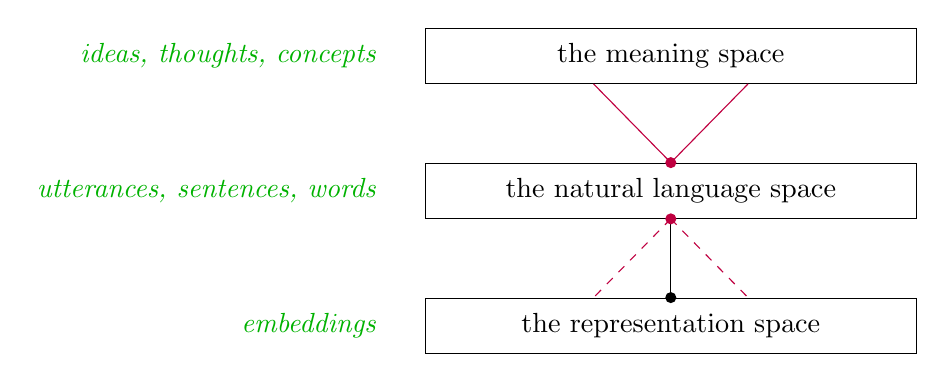
\begin{tikzpicture}[
	space/.style = {text width=60mm,  align=center, draw},
	pointdot/.style = {fill=purple, circle, minimum size=4pt,text width=0mm, inner sep=0pt},
	obj/.style = {font={\itshape}, green!70!black}		
	]
	\node[space](idea){the meaning space};
	\node[obj, left = 0.5 of idea]{ideas, thoughts, concepts};
	
	\node[space, below = of idea](nl){the natural language space};
	\node[obj, left = 0.5 of nl]{utterances, sentences, words};
	
	\node[space, below = of nl](emb){the representation space};
	\node[obj, left = 0.5 of emb]{embeddings};
	% Objects: Embeddings
	
	\draw[purple] (idea.200) to (nl.north);
	\draw[purple] (idea.-20) to (nl.north);
	\node[pointdot] at (nl.north) {};
	
	\draw[] (nl) to (emb);
	\draw[dashed,purple] (nl.south) to (emb.20);
	\draw[dashed,purple] (nl.south) to (emb.-200);
	\node[pointdot] at (nl.south) {};
	
	\node[pointdot,black] at (emb.north) {};
	
	\end{tikzpicture}
	\caption{\label{fig:spaces} The representation space is a computationally manipulate representation of the meaning space.
	The natural language utterances come from points in the meaning space; 
	though due to ambiguity we can only truly hope to estimate distributions over meanings when interpreting them.
	A single point embedding is an approximation to a distribution with a single tight peak.
 }
\end{figure}

We can consider that there is a true semantic space of ideas: a meaning space.
When speaking, this space is projected down to a natural languages space,
which we represent using an embedding in the representation space, with the hope that this representation can be related to the meaning space.
This is shown in the diagram in \Cref{fig:spaces}.

To quote \citet{webster}:  ``A sentence is a group of words expressing a complete thought.'', it is not a complete thought, only the \emph{expression} of one.
This projection from idea (the meaning space) to utterance (the natural language space) is imperfect -- it is lossy.
Many ideas are expressed the same way, and language thus has a lot of ambiguity.
When we try to understand the meaning of a natural language utterance we are trying to find the point in the meaning space that the speaker intends.
Some times the natural language space alone is enough to recover a good idea of the point in the meaning space the speaker intends,
but other times it is not.

The preimage\footnote{I say preimage in an abuse of mathematical terminology.} of a point in the natural language space (e.g. a sentence),
is a probability distribution over the meaning space that could have lead to that utterance, $P(meaning \mid utterance)$.
This distribution could be combined with other factors (in a Bayesian way); either from that natural language context, or the environment more broadly.
For example, to use a meaning that centres around word sense:
we can identify two (of the many) senses of the word \natlang{apples}:
one in reference to the fruit, the other in reference to the computers.
Thus, on its own the sentence \natlang{Apples are good.}
suggests a distribution with at least two peaks in the meaning space.
Combine that utterance, with the context of being in a computer store, rather than a grocer, and the probability of one of the two peaks can be increased, though the other not entirely removed.
Further around each peak remains adjacent closely related possible meanings.
For example the statement could be in relation to only computers, or also to other products.
the meaning space is a continuous space, with every thought corresponding to a unique point. It is an uncountably large space.
In contrast the natural language space is countably large, being composed of finite length combinations of symbols taken from a finite alphabet.
An uncountable number of points in the meaning space are projected down to a single point in a natural language space.


An embedding space is a particular instance of a representation space, 
much like the English language is a particular instance of a natural language space.
When designing an embedding method (for sentences, words or other structures),
we seek to define a representation space
that has good properties for reflection relationships in the meaning space in a way that is computationally manipulatable using simple operations (like sums).
In particular it should have a continuous mapping to and from the meaning space.
A neighbourhood in the representation space, should correspond to a neighbourhood in the meaning space.
\Cref{SentVecMeaning} investigates this for sentence embeddings.
This is done by taking points in the natural language space known to come from very nearby points in the meaning space, that is to say paraphrases,
and then checking that they belong to nearby points in the embedding space.


As each point in the natural language space defines a distribution over the meaning space of what may be meant;
and the representation space is attempting to be in correspondence to the meaning space;
it is such that each point in the natural language space should project to a distribution over the embedding space.
Instead, most methods project natural language points to single points in embeddings space.
This is viable when the region in the meaning space that the utterance (natural language point) could have come from is small -- in particular when the distribution in the meaning space has narrow variance and is mono-modal.
In that case the single point estimate in the embedding space is an useful approximation.


This has particularly clear utility for word sense embeddings,
which are defined by multimodal distributions,
with large peaks for each homonym, and smaller nearby peaks for each polyseme.
Furthermore we can't rule out the speaker using the word incorrectly or metaphorically, which gives rise to nonzero values elsewhere in the meaning space.
Word-sense embeddings produce multiple sense embeddings -- ideally one corresponding to each peak in the meaning space.
We know these peaks are only rough approximations to the true point in the meaning space for a given usage of a word.
\Cref{RefittingSenses} attempts to find other points in the embeddings space, that better corresponds to the true point in the meaning space for the particular use.
These will be near those peaks given by the point estimates from the senses found using word sense induction.
The refitting method (discussed in \Cref{RefittingSenses}) efficiently interpolates a point between those peaks based on likelihood.


Unsupervised methods, in particular word embeddings (though it applies also more generally), are ungrounded.
They are based only on the natural language space observations.
The goal is not to capture meaning in this space,
but rather to create a space that is a good input to a supervised system that can learn a good correspondence from the natural language space to the meaning space. 
While we would not normally think of the SOWE sentence representation space as one for which there would be an easy alignment to the meaning space,
\Cref{SentVecMeaning} shows that it is.
A strong point in its favour is that it directly benefits from word embeddings.
While themselves ungrounded, word embeddings are excellently suited for creating a representation space, as they have an internal consistency which makes it easy to apply supervision to give grounded meaning representations.
It's great strength comes from Firth's distributional hypothesis, that words occurring in similar contexts have similar meaning.
While this does not allow the encoding of meaning itself, it does allow the encoding of similarity of meaning.
This is ideally suited for creating a space that will make a good source representation for a supervised method applied for natural language understanding task on words.
Were that task accomplished with a neural network, the later hidden layers, or the fine-turned embeddings would form a grounded representation of the meaning space.
Our results show that that strength is carried forth into linear combinations of such embeddings.


The color understanding task considered in \Cref{ColorEst} is interesting.
It is a typical natural language understanding system,
which takes a point in a natural language space (a color name),
moves through a representation space (the output of one of the input modules: SOWE, CNN, or RNN) using supervision to output something from a meaning space.
Notably however, the meaning space is \emph{very well grounded} to the HSV color space.
We can, for many purposes, say for this natural language understanding task, the color space \emph{is} the meaning space.
Using point estimation it outputs a point in the meaning space, reflecting (in some sense) the most reasonable guess of the meaning.
Using distribution estimation it outputs a distribution over the meaning space, fully reflecting the knowledge we have to infer the meaning.
The fact that even on the subset of the testing data where word order was ambiguous, SOWE was the best performing model highlights an important notion.
Word order ambiguity is just one amongst many sources of ambiguity in any representation of natural language.
In the color case, it boils down to the additional ambiguity of being unable to encode the word order difference between \natlang{bluish green} and \natlang{greenish blue} being negligible compared to the inherent ambiguity in the meaning of either.
Both phrases give rise to a large and overlapping distribution across the meaning space.

In cases where there are multiple reasonable word orderings,
this means that multiple points in the true meaning space, correspond to a single point in the representational LCOWE space.
However, this is not exceptional: 
many sentences have two or more interpretations, a humorous example being an accidental pun.
Thus even in a representation space that fully captures the natural language features,  a single point in that representation space
corresponds to two points in the meaning space;
as the single point in the natural language space could have come from either point in the meaning space.
As such, ambiguity from loss of word order is not an unique and unsalvageable problem.
If we thus had a distribution over the meaning space, corresponding to the interpretation of a SOWE, it would have two peaks corresponding to two different word orders.
While such a discussion is purely theoretical as we do not have any way to generate such a distribution over true the meaning space,
it remains interesting for cases where we have a space that we can treat as being the meaning space (e.g. the HSV space for colors).
As we can use other contextual information to define a prior and thus decrease distributions associated with other ambiguities,
we can use language models to provide a prior over those peaks; based on the likelihood of word orders.
There exists a trivial extension of the work presented in \Cref{BOWgen,SOWE2Sent}, where the mixed integer programming model is constrained to give the second (and so forth) most likely solution, together with it's probability.
It is however not computationally practical, nor useful without a better the meaning space representation.


While the research presented in this dissertation has made use of the idea that we are working with a sample from a distribution over a proxy for the meaning space,
it is our belief that further advancements would benefit from fully considering
word embeddings and other objects from the representation spaces, not as discrete points but as random variables with a linked distribution.
This however comes with significant challenges in that manipulating the very high dimensional distributions that are required for this is computationally challenging.



\todo{Where does this paragraph belong?}
\Cref{SentVecMeaning} and \Cref{ColorEst} both consider represent contagious linguistic structures -- sentences and shore phrases respectively, as input representations.
\Cref{SentVecMeaning} directly explores the ability to find regions of representation space that match to regions of meaning space.
Further, the output of the output modules discussed in \Cref{ColorEst} are a grounded the representation space, though that work did not examine it directly.
\Cref{RefittingSenses} considers the representation of word senses, and it navigates this the representation space to find new representations which better describe a particular use of a word.
\Cref{NovelPerspective} is more atypical:
the features sets considered for the point of view detection task,
characterize how a particular named entity token was used throughout a chapter.
It is thus not a representation of the chapter meaning, as it varies for the different named entities.
It is in fact a representation of how that named entity is related to the events described in the chapter.
It seems like the MOWE feature set used in \Cref{NovelPerspective} it is vastly insufficient to represent such information given it is only a mean of the immediately adjacent words -- nothing like the whole chapter's contents.
However, as was demonstrated by the classical feature set considered in the same chapter, which primarily consisted of adjacent part of speech tag counts, and which also achieved very good results, surface information encodes a surprising amount of semantic depth.


\end{document}